%% CAMERA-READY (accepted 2026-08-23 as PROMPTOPS 2026 paper 16; CR deadline 1 Sep 2026 per the
%% 2026-08-24 follow-up email, page limit strictly 8 INCLUDING references per the same email).
%% [review,anonymous] dropped and the author block added for the camera-ready; the rights block
%% (\setcopyright, DOI, ISBN, \acmSubmissionID) is inserted with the owner when the author-kit /
%% ACM rights email arrives. Until then \setcopyright{none} + printacmref=false are placeholders,
%% the same interim state paper 195 used before its rights confirmation.
\documentclass[sigconf,screen]{acmart}
% Suppress /PTEX.FileName comments in the PDF: they carry the include path of every figure into
% the shipped bytes, which is how a username reached a published PDF once (LEARNINGS BN3).
\pdfsuppressptexinfo=-1

\AtBeginDocument{%
  \providecommand\BibTeX{{\normalfont B\kern-0.5em{\scshape i\kern-0.25em b}\kern-0.8em\TeX}}}
% MEASURED INERT 2026-08-31, kept only so a future reader does not re-add it believing it works:
% acmart's \maketitle sets the page style itself, so a \pagestyle in the PREAMBLE has no effect
% (BH5's remedy for a fabricated running head requires \pagestyle AFTER \maketitle). Built both
% ways: 8 pages, 0 errors, rendered text byte-identical. The camera-ready WANTS acmart's standard
% running head, because the venue string is now real and fetched, so nothing here needs suppressing.
\pagestyle{plain}

% RIGHTS BLOCK. Supplied by the ACM eRights system for paper asews26povcmain-p16-p and inserted
% VERBATIM on 2026-08-31. Do not retype, reflow or "correct" any string in it: the publisher's
% block supersedes the venue's own web branding and this file's earlier fetched strings
% (LEARNINGS BN4, BO15). Two consequences worth knowing before editing anything below.
%   1. The ACM proceedings title is "Proceedings of the 1st International Workshop on PromptOps
%      and Vibe Coding", which is NOT the workshop's web branding ("PROMPTOPS 2026: Engineering
%      Reliable AI-Augmented Software Development") that this file carried through review. Both
%      are real strings for different objects; the rights system is authoritative for the
%      proceedings, so consistency.py now asserts equality with THESE strings and its old
%      "International Workshop on must not appear" clause has been retired.
%   2. \setcopyright{cc} + \setcctype{by} pull the doclicense CC badge as an included PDF, whose
%      absolute path pdfTeX would otherwise write into the shipped bytes as /PTEX.FileName. That
%      is the LEARNINGS BN3 username leak; \pdfsuppressptexinfo=-1 above prevents it and
%      papertools/pdf_production_check.py verifies the bytes after every build.
% Unchanged and still fetched facts: dates October 12-16 2026, Munich Germany; page limit strictly
% 8 INCLUDING references (2026-08-24 chairs' email, re-confirmed on the venue page 2026-08-31).
\copyrightyear{2026}
\acmYear{2026}
\setcopyright{cc}
\setcctype{by}
\acmConference[POVC '26]{Proceedings of the 1st International Workshop on PromptOps and Vibe Coding}{October 12--16, 2026}{Munich, Germany}
\acmBooktitle{Proceedings of the 1st International Workshop on PromptOps and Vibe Coding (POVC '26), October 12--16, 2026, Munich, Germany}
\acmDOI{10.1145/3843779.3844636}
\acmISBN{979-8-4007-2991-1/2026/10}

\usepackage{booktabs}
\usepackage{balance}
\usepackage{enumitem}
\usepackage{graphicx}
\usepackage{xspace}
% Every generated macro ends in \xspace. Without it LaTeX swallows the space that terminates a
% control-sequence name, so "\PctDrift points" renders as "43.8points". The build log is clean
% either way, which is why this is enforced by the gate and checked again on the rendered text.
\xspaceaddexceptions{\% ] \\ }
% \lit marks a number quoted from a cited source, so the build gate can tell it apart from one of
% ours, every one of which must come from a generated macro.
\newcommand{\lit}[1]{#1}

% GENERATED by code/make_macros.py. Do not edit by hand.
% Every number in the manuscript resolves through one of these.
\newcommand{\PaperTitle}{Your Prompt Is Only Half the Prompt: Silent Chat-Template Drift in Open-Weight Model Repositories}
\newcommand{\NCandidates}{1000\xspace}
\newcommand{\NIncludedTotal}{618\xspace}
\newcommand{\NFrame}{400\xspace}
\newcommand{\NGated}{41\xspace}
\newcommand{\NNoTemplateFile}{205\xspace}
\newcommand{\NNoTemplateRev}{136\xspace}
\newcommand{\NDrifted}{175\xspace}
\newcommand{\PctDrifted}{43.8\xspace}
\newcommand{\NBehavioural}{103\xspace}
\newcommand{\PctBehFrame}{25.8\xspace}
\newcommand{\PctBehDrifted}{58.9\xspace}
\newcommand{\NBehSettled}{34\xspace}
\newcommand{\PctBehSettledFrame}{8.5\xspace}
\newcommand{\NBehWeightSilent}{79\xspace}
\newcommand{\PctBehWeightSilent}{76.7\xspace}
\newcommand{\NFixtures}{30\xspace}
\newcommand{\PctBehSettledNoFix}{6.5\xspace}
\newcommand{\PctEventsBehNoFix}{47.2\xspace}
\newcommand{\NEvents}{289\xspace}
\newcommand{\NEventsDecidable}{273\xspace}
\newcommand{\NEventsUndecidable}{16\xspace}
\newcommand{\NEventsBeh}{137\xspace}
\newcommand{\PctEventsBeh}{50.2\xspace}
\newcommand{\NEventsCosmetic}{136\xspace}
\newcommand{\NEventsWeightSilent}{233\xspace}
\newcommand{\PctEventsWeightSilent}{80.6\xspace}
\newcommand{\MedianDaysFirstChange}{1.5\xspace}
\newcommand{\SettledDays}{30\xspace}
\newcommand{\MaxDistinctTemplates}{9\xspace}
\newcommand{\NOutOfFrame}{218\xspace}
\newcommand{\PctOOFDrifted}{34.4\xspace}
\newcommand{\PctOOFBeh}{17.4\xspace}
\newcommand{\ProbeUserOnly}{116\xspace}
\newcommand{\ProbeGenpromptTrue}{116\xspace}
\newcommand{\ProbeGenpromptFalse}{113\xspace}
\newcommand{\ProbeMultiTurn}{84\xspace}
\newcommand{\ProbeSystemUser}{81\xspace}
\newcommand{\ProbeContract}{81\xspace}
\newcommand{\NValidated}{7\xspace}
\newcommand{\NValidatedFailed}{0\xspace}
\newcommand{\NaiveAlerts}{289\xspace}
\newcommand{\RenderAlerts}{137\xspace}
\newcommand{\SuppressedAlerts}{136\xspace}
\newcommand{\PctSuppressed}{49.8\xspace}
\newcommand{\NStranded}{99\xspace}
\newcommand{\MedianDaysStranded}{1.7\xspace}
\newcommand{\CostComputeMs}{9.2\xspace}
\newcommand{\NProbes}{6\xspace}
\newcommand{\MedAbsLenCosmetic}{52\xspace}
\newcommand{\MedAbsLenBehavioural}{86\xspace}
\newcommand{\MaxCosmeticLenChange}{4403\xspace}
\newcommand{\NBehZeroLenChange}{5\xspace}
\newcommand{\DiffAUC}{0.57\xspace}
\newcommand{\NExecEpisodes}{1260\xspace}
\newcommand{\NExecTruncated}{4\xspace}
\newcommand{\NExecRenderErrors}{120\xspace}
\newcommand{\NCheckpoints}{5\xspace}
\newcommand{\FloorDSCoder}{90.0\xspace}
\newcommand{\NVersDSCoder}{6\xspace}
\newcommand{\ResDSCoderA}{40.0\xspace}
\newcommand{\ConDSCoderA}{98.3\xspace}
\newcommand{\ResDSCoderB}{43.3\xspace}
\newcommand{\ConDSCoderB}{98.3\xspace}
\newcommand{\ResDSCoderC}{43.3\xspace}
\newcommand{\ConDSCoderC}{96.7\xspace}
\newcommand{\ResDSCoderD}{45.0\xspace}
\newcommand{\ConDSCoderD}{95.0\xspace}
\newcommand{\ResDSCoderE}{45.0\xspace}
\newcommand{\ConDSCoderE}{98.3\xspace}
\newcommand{\ResDSCoderF}{45.0\xspace}
\newcommand{\ConDSCoderF}{98.3\xspace}
\newcommand{\FloorLlama}{26.7\xspace}
\newcommand{\NVersLlama}{3\xspace}
\newcommand{\ResLlamaA}{43.3\xspace}
\newcommand{\ConLlamaA}{100.0\xspace}
\newcommand{\ResLlamaB}{43.3\xspace}
\newcommand{\ConLlamaB}{100.0\xspace}
\newcommand{\ResLlamaC}{43.3\xspace}
\newcommand{\ConLlamaC}{100.0\xspace}
\newcommand{\FloorMistral}{0.0\xspace}
\newcommand{\NVersMistral}{2\xspace}
\newcommand{\ResMistralA}{0.0\xspace}
\newcommand{\ConMistralA}{0.0\xspace}
\newcommand{\ResMistralB}{28.3\xspace}
\newcommand{\ConMistralB}{100.0\xspace}
\newcommand{\FloorPhi}{0.0\xspace}
\newcommand{\NVersPhi}{3\xspace}
\newcommand{\ResPhiA}{21.7\xspace}
\newcommand{\ConPhiA}{90.0\xspace}
\newcommand{\ResPhiB}{10.0\xspace}
\newcommand{\ConPhiB}{45.0\xspace}
\newcommand{\ResPhiC}{23.3\xspace}
\newcommand{\ConPhiC}{88.3\xspace}
\newcommand{\FloorQwen}{15.0\xspace}
\newcommand{\NVersQwen}{2\xspace}
\newcommand{\ResQwenA}{28.3\xspace}
\newcommand{\ConQwenA}{40.0\xspace}
\newcommand{\ResQwenB}{28.3\xspace}
\newcommand{\ConQwenB}{40.0\xspace}
\newcommand{\ShortMistral}{Mistral-7B-Instruct-v0.2\xspace}
\newcommand{\ShortPhi}{Phi-3-mini-4k-instruct\xspace}
\newcommand{\ShortDS}{deepseek-coder-6.7b-instruct\xspace}
\newcommand{\ShortQwen}{Qwen2.5-7B-Instruct\xspace}
\newcommand{\ShortLlama}{Meta-Llama-3-8B-Instruct\xspace}
\newcommand{\MaxNoiseFloor}{90.0\xspace}
\newcommand{\MinNoiseFloor}{0.0\xspace}
\newcommand{\NTasksExec}{60\xspace}
\newcommand{\NFamily}{18\xspace}
\newcommand{\NUninformative}{5\xspace}
\newcommand{\NSigRes}{1\xspace}
\newcommand{\NSigContract}{3\xspace}
\newcommand{\MistralRenderErr}{60\xspace}
\newcommand{\MistralPHolmRes}{0.0003\xspace}
\newcommand{\MistralPHolmCon}{<0.0001\xspace}
\newcommand{\PhiCIDownLo}{5.0\xspace}
\newcommand{\PhiCIDownHi}{20.0\xspace}
\newcommand{\PhiCIUpLo}{-21.7\xspace}
\newcommand{\PhiCIUpHi}{-5.0\xspace}
\newcommand{\MistralCILo}{-40.0\xspace}
\newcommand{\MistralCIHi}{-16.7\xspace}
\newcommand{\PhiPHolmConDown}{<0.0001\xspace}
\newcommand{\PhiPHolmConUp}{<0.0001\xspace}
\newcommand{\PhiPHolmResDown}{0.250\xspace}
\newcommand{\PhiPHolmResUp}{0.133\xspace}
\newcommand{\PhiFirstLastRes}{1.00\xspace}
\newcommand{\NAllPairs}{23\xspace}
\newcommand{\NAllSigRes}{1\xspace}
\newcommand{\NAllSigCon}{3\xspace}
\newcommand{\FloorDiscDSCoder}{4\xspace}
\newcommand{\FloorDiscLlama}{1\xspace}
\newcommand{\FloorDiscMistral}{0\xspace}
\newcommand{\FloorDiscPhi}{0\xspace}
\newcommand{\FloorDiscQwen}{6\xspace}
\newcommand{\QwenFloorP}{0.031\xspace}
\newcommand{\MistralDisc}{17\xspace}
\newcommand{\PhiDiscDown}{7\xspace}
\newcommand{\PhiDiscUp}{8\xspace}
\newcommand{\NMarkersChecked}{4\xspace}
\newcommand{\MarkerMinRatio}{1.7\xspace}
\newcommand{\NSFEpisodes}{420\xspace}
\newcommand{\NSFRenderErrors}{0\xspace}
\newcommand{\NSFFamily}{3\xspace}
\newcommand{\NSFSigRes}{0\xspace}
\newcommand{\NSFSigCon}{0\xspace}
\newcommand{\SFFloorMistral}{0.0\xspace}
\newcommand{\SFResMistralA}{28.3\xspace}
\newcommand{\SFConMistralA}{100.0\xspace}
\newcommand{\SFResMistralB}{28.3\xspace}
\newcommand{\SFConMistralB}{100.0\xspace}
\newcommand{\SFFloorPhi}{3.3\xspace}
\newcommand{\SFResPhiA}{23.3\xspace}
\newcommand{\SFConPhiA}{95.0\xspace}
\newcommand{\SFResPhiB}{23.3\xspace}
\newcommand{\SFConPhiB}{95.0\xspace}
\newcommand{\SFResPhiC}{21.7\xspace}
\newcommand{\SFConPhiC}{93.3\xspace}
\newcommand{\NHealthyTemplates}{3\xspace}
\newcommand{\MaxHealthyResShift}{1.7\xspace}
\newcommand{\MaxHealthyConShift}{5.0\xspace}
\newcommand{\NHistChecked}{16\xspace}
\newcommand{\NHistMismatch}{0\xspace}
\newcommand{\NDSPairs}{14\xspace}
\newcommand{\DSMinP}{1.00\xspace}


\begin{document}

\title{\PaperTitle}

\author{Simarjot Khanna}
\affiliation{%
  \institution{Independent Researcher}
  \country{Canada}
}
\email{simarkhanna76@gmail.com}

\begin{abstract}
PromptOps treats prompts as code: versioned, reviewed, and defended by a regression suite. The
prompt a model actually reads is not the prompt a team writes. It is first rewritten by the model's
\emph{chat template}, an executable Jinja program shipped inside the model repository, edited in
place, with no version of its own. How often this hidden dependency changes, and with what
behavioural consequence, has not been measured. We reconstruct the default-branch template history
of \NFrame{} of the most-downloaded text-generation repositories on the Hugging Face Hub. A
renderer validated byte-for-byte against the reference implementation decides whether each edit
changes what the model is shown, and we run \NCheckpoints{} local checkpoints under their own
repositories' historical templates. \PctDrifted\% of the repositories changed their template after
first publishing one, and \PctEventsWeightSilent\% of the change events moved no weight file,
invisible to a team that pinned the model and verified its weights; \PctEventsBeh\% of the
decidable edits change what the model is shown. Much of the raw rate is launch-week churn, and we
report the settled figure beside it: \PctBehSettledFrame\% of the frame saw such an edit land more
than \SettledDays{} days after its first template. In a one-repository case study, an
edit that dropped the system role halved output-contract compliance from \ConPhiA\% to \ConPhiB\%
until a later edit largely restored it. \textsc{templatelock} pins what a template renders rather than
what it says, separating the edits that matter from the ones that do not at \CostComputeMs{} ms per
model. Until prompt pipelines version the template, pinning the prompt and the model does not pin
the model's input.

\end{abstract}

\begin{CCSXML}
<ccs2012>
<concept>
<concept_id>10011007.10011074.10011099</concept_id>
<concept_desc>Software and its engineering~Software verification and validation</concept_desc>
<concept_significance>500</concept_significance>
</concept>
<concept>
<concept_id>10011007.10011006.10011071</concept_id>
<concept_desc>Software and its engineering~Software configuration management and version control systems</concept_desc>
<concept_significance>500</concept_significance>
</concept>
</ccs2012>
\end{CCSXML}
\ccsdesc[500]{Software and its engineering~Software verification and validation}
\ccsdesc[500]{Software and its engineering~Software configuration management and version control systems}

\keywords{PromptOps, chat templates, prompt versioning, drift detection, open-weight models,
reproducibility}

\maketitle

\section{Introduction}

PromptOps asks software teams to treat prompts as code: version them, review them, put them under
test, and gate releases on a prompt regression suite. The premise is that if the prompt is pinned
and the model is pinned, the system is pinned.

It is not. Between the prompt a team writes and the tokens a model reads sits a second artifact that
neither pin covers. Open-weight chat models ship a \emph{chat template}: a Jinja program,
stored inside the model repository, that rewrites a list of messages into the exact string the model
is served. It decides where the system message goes, or whether it survives at all; it decides which
control tokens delimit a turn; it decides what is appended to invite the assistant to speak. Change
it and the model sees different input, even though the prompt is byte-identical and the weights have
not moved.

That artifact is edited in place. It lives on a repository's default branch with no version of its
own, so a team that pulls a model by name gets whichever template happened to be committed most
recently. There is no semantic version to pin, no changelog convention, and no equivalent of the
package-manager machinery that at least records when a dependency moved. The npm ecosystem has
version numbers and breaking changes still reach clients through releases that were supposed to be
backward compatible~\cite{venturini2023depended}. Chat templates do not have the version numbers.

The hazard of a mismatched template was named when the mechanism
shipped~\cite{carrigan2023chattemplates}; how often the template itself moves, and to what effect,
has not been measured. That is the gap this paper closes, with three research questions.
\textbf{RQ1:} how often does the chat template of a popular open-weight repository change after
release, and how much of that change is invisible to a team that pins the model and verifies its
weights? \textbf{RQ2:} when the template changes, does the model's behaviour follow? \textbf{RQ3:}
can a check tell the edits that change the model's input from the edits that do not, cheaply enough
to run in every build? To answer them we reconstruct the default-branch history of every chat
template in a frame of \NFrame{} of the most-downloaded text-generation repositories on the Hugging
Face Hub. We decide which edits actually change what a model is shown by \emph{rendering} rather
than by reading the Jinja source, and we then hold a checkpoint and a conversation fixed while
varying only the template.\footnote{Artifact: \url{https://github.com/s1mar/chat-template-drift}}

The question matters most for exactly the practice this workshop is named after. A developer
prompting a model and judging the result by running it~\cite{fawzy2026verification} has no way to
separate a model that has become worse from a prompt wrapper that changed underneath. A grey-literature
review of \lit{101} practitioner sources finds that quality assurance in this style of work is
frequently skipped altogether~\cite{fawzy2026vibepractice}, which leaves the template free to move
without anyone noticing.

\paragraph{Contributions.}
\begin{itemize}[leftmargin=*,itemsep=1pt,topsep=2pt]
\item The first empirical measurement of chat-template drift (RQ1). In a frame of \NFrame{}
  repositories, \PctDrifted\% changed their chat template after first publishing one, and
  \PctEventsWeightSilent\% of change events occurred in an interval where no model-weight file
  moved.
\item A rendering-based test that separates cosmetic edits from behavioural ones (RQ1), validated
  byte-for-byte against the reference implementation. It shows that \PctEventsBeh\% of decidable
  change events alter what the model is shown, and that textual diff size does not predict which.
\item An execution-grounded study over \NCheckpoints{} checkpoints run under their own repositories'
  historical templates, with a replication control that establishes the noise floor (RQ2). Its
  strongest effect, an edit that halves output-contract compliance, comes from one repository and is
  scoped as a case study throughout.
\item \textsc{templatelock}, a check that pins a template by what it renders rather than by its
  text (RQ3). Replayed over the frame it raises \RenderAlerts{} alerts where a plain hash raises
  \NaiveAlerts{}, and it costs \CostComputeMs{} ms per model.
\end{itemize}

\section{The chat template is executable code}

A chat model is trained on a specific serialisation of dialogue. Serving it a differently
serialised conversation is out of distribution, so the serialisation is shipped with the model. In
the Hugging Face ecosystem it is the \texttt{chat\_\allowbreak template} field of
\texttt{tokenizer\_\allowbreak config.\allowbreak json}, or a sibling
\texttt{chat\_\allowbreak template.\allowbreak jinja}, and it is applied by
\texttt{apply\_\allowbreak chat\_\allowbreak template}~\cite{hfchattemplating}.

Three properties make it a supply-chain artifact rather than a configuration detail. It is
\emph{executable}, being a Jinja program with conditionals and loops rather than a format string. It
is \emph{invisible at the call site}: application code passes a message list and never sees the
rendered result. And it is \emph{unversioned}: it has no identity separate from the repository
revision that carries it, so pinning it means pinning a commit, which the common tooling paths do
not do by default.

The failure this creates is specific. A prompt suite that asserts properties of a model's reply will
happily re-run after a template edit, exercise a different serialisation, and report whatever it
finds as a property of the prompt.

\section{Study design}

The design, the frame, the definitions and a falsification criterion were fixed in advance and are
part of the released artifact. Each element of the design serves one research question: the frame
and the change taxonomy serve RQ1, the execution arms and their controls serve RQ2, and the
replayed check serves RQ3; Sections~\ref{sec:rq1}, \ref{sec:rq2} and \ref{sec:check} answer them in
that order.

\subsection{Frame}

We list Hub models with \texttt{pipeline\_tag = text-generation} in descending all-time downloads
as recorded on 2026-07-30, the day the frame was drawn, and take them in order. A repository is included if an anonymous clone succeeds and at least one
default-branch revision carries a chat template. The frame is the first \NFrame{} repositories that
qualify, drawn from \NCandidates{} candidates. Of those candidates, \NIncludedTotal{} qualified,
\NNoTemplateFile{} never carried a template-bearing file, \NNoTemplateRev{} carried the file but
never a template in it, and \NGated{} were gated or absent. No candidate is unaccounted for. The
\NOutOfFrame{} repositories that qualified beyond rank \NFrame{} are held out and reported
separately; they are never merged into the frame.

History is reconstructed with one blob-filtered, single-branch clone per repository (the collector
in the released package), after which the
whole commit graph is read locally. Model weights are Git LFS objects and are never fetched.

\subsection{What counts as a change, and as a silent one}

A \emph{template revision} is a default-branch commit at which the extracted template string differs
from the previous one. A repository has \emph{drifted} if it exhibits at least two distinct
templates, which is to say the template you get depends on when you pulled.

An interval between consecutive template revisions is \emph{weight-silent} if no tracked
model-artifact file changed in it. This is the case that defeats ordinary diligence: a team that
pinned the model by name and verified its weights would have seen nothing at all.

\subsection{Cosmetic or behavioural, decided by rendering}

Reading a Jinja diff is a poor way to decide whether an edit matters, because a large reformatting
can be inert and a four-character edit can drop the system message. We decide it by rendering. Six
probe conversations, fixed in advance, are rendered through both templates: a single user turn;
system plus user; a four-message multi-turn exchange; a turn with the generation prompt requested
and one without; and a system message carrying an output-contract instruction. A pair is
\emph{behavioural} if any probe renders differently, or if one template renders a probe that the
other refuses. A pair is \emph{cosmetic} if every probe is byte-identical, however large the textual
diff. A pair where \emph{neither} template renders a probe is \emph{undecidable} for that probe, and
a pair with no decidable probe is excluded from the split and counted in its own right.

That third category is not fastidiousness. An early version of this analysis folded both-failed into
``identical'', a missing import made every render fail, and the pipeline reported zero behavioural
changes out of \NEvents{} with no error anywhere. A category that can absorb total instrument
failure and still present as a clean null must not exist. The \NEventsUndecidable{} undecidable
events that do occur have three concrete causes, and in every one both members of the pair fail.
Some templates are written against a nonstandard Jinja extension tag (\texttt{generation}) that
the sandboxed Jinja environment pinned for this study rejects. Others fail to parse at either revision: in one repository
a stretch of consecutive revisions carries the same parse error, commits titled as fixes
(``fix typo with missing closing curly bracket'') still left the template unparseable, and by
definition only a revision that renders again can make a pair decidable. A few templates include a
companion template file that our loader-free sandbox cannot resolve. The first and third causes
are limits of our renderer; the second is what a repair in progress looks like from outside the
repository. All \NEventsUndecidable{} are excluded by the rule above: a pair with no decidable
probe is not scored.

\paragraph{Renderer validation.} Every behavioural claim rests on our renderer agreeing with the one
practitioners actually run. Before any measurement was believed, our renderer was required to equal
the reference \texttt{apply\_\allowbreak chat\_\allowbreak template} byte for byte on every probe of
every repository in a fixed list of eight reference checkpoints. It does, on the \NValidated{}
whose tokenizers load in our pinned environment; the eighth needs a tokenizer backend outside it. A renderer that silently differed would manufacture divergence, which is the direction that
flatters this paper.

Checking current templates leaves a gap, because the study renders \emph{historical} ones. We close
it rather than bound it: the Hub serves any revision, so for each of the \NHistChecked{} templates
used as an execution arm below (one arm is one historical template a checkpoint is run under) we
load that revision's own tokenizer and compare its
\texttt{apply\_\allowbreak chat\_\allowbreak template} against ours on the same probes.
\NHistMismatch{} of the \NHistChecked{} mismatch. The same check confirms that the template we extracted from the commit
graph is the one the reference implementation loads at that revision, so both the extraction and the
rendering are validated on exactly the inputs the results depend on.

\subsection{Execution: same weights, same conversation, different template}
\label{sec:exec}

Mining shows that renderings change. Whether the model cares is a different question, and the
only way to answer it is to run the model.

We use \NCheckpoints{} local checkpoints, each paired with the Hub repository whose template
history it is served under: Qwen2.5-7B-Instruct, Phi-3-mini-4k-instruct,
deepseek-coder-6.7b-instruct, Mistral-7B-Instruct-v0.2, and Meta-Llama-3-8B-Instruct. They were
selected as widely deployed open-weight instruction-tuned models with reconstructable template
histories at the time of the study; every RQ2 comparison is within-checkpoint, so checkpoint
generation is not a confound of any comparison. For each checkpoint we take its
repository's render-distinct historical templates, render an identical repair conversation through
each, and send the rendered string to the same local weights through a local Ollama endpoint whose
raw mode bypasses the
server's own templating. The conversation, the decoding parameters, the seed, the stop tokens and
the weights are identical in every arm. The rendered prompt string is the only thing that differs.

The task is single-function program repair over a seeded sample of \NTasksExec{} tasks from the
code-repair split of HumanEvalPack~\cite{muennighoff2024octopack}, graded by executing the task's
own test. An episode is one task sent once under one template arm; decoding is greedy (temperature
zero) with a 1536-token generation cap, on the quantised builds
named, with their digests, in the artifact. Identical rendered prompts are served from a
generation cache, so two arms that render a conversation identically receive the same stored
reply; the replication arms are keyed separately, so a floor is always a fresh generation. The cap
truncates \NExecTruncated{} replies, all retained and
scored. We record whether the returned program passes, whether the reply obeyed the
stated output contract, and a hash of the reply. The contract is the system message's closing
instruction, ``Reply with exactly one fenced python code block and no other text''; a reply
complies if it contains exactly one fenced block and that block defines the task's entry point.

\paragraph{The noise floor.} Greedy decoding on a GPU is not perfectly reproducible, so a divergence
rate means nothing without knowing what zero looks like. Each checkpoint therefore runs its first
template a second time, byte-identical prompt and settings, and the divergence between those two
runs is the floor against which every cross-template comparison is read. We report each checkpoint's
replication discordance next to its cross-template discordance, so a difference no larger than the
checkpoint's own noise cannot be mistaken for an effect.

\paragraph{Does the transport preserve the template?} Sending an already-rendered string risks the
server re-tokenising the template's control markers as ordinary text, which would mean we were
measuring our own plumbing. We test it directly rather than assume it. Each checkpoint's own marker
is submitted twice, once intact and once with its characters separated, and on all
\NMarkersChecked{} checkpoints checked the separated characters cost at least \MarkerMinRatio{}
times as many tokens as the intact marker, so no marker is being shattered into its characters. On \ShortQwen{} and
on \ShortPhi{}, the checkpoint carrying the behavioural result below,
the server's token count for the marker equals the reference tokenizer's exactly. The two other
checkpoints differ from the reference by one token on a marker measured in isolation, \ShortMistral{}
and \ShortLlama{}, and neither bears on a claim: \ShortMistral's effect is a rendering exception
raised before a single token exists, and \ShortLlama{} yields no informative comparison at all.
\ShortDS{}, whose comparisons all fail to reject,
uses no bracketed marker and is not part of this
probe. This is a bound rather than a proof of identical token identifiers, which the server does not
expose.

\subsection{Analysis}

All comparisons are paired over tasks, since every arm sees every task. Paired binary outcomes use
McNemar's exact test on the discordant pairs; intervals are percentile bootstraps over tasks with
10{,}000 resamples. Multiplicity is corrected with Holm over the family of every informative
within-checkpoint pair, separately for each outcome. The family contains both the consecutive
transitions and the first-versus-last comparisons, so both kinds are corrected and reported, not
only the one that suits the argument.

\section{RQ1: how often, and how silently}
\label{sec:rq1}

% GENERATED by code/tables.py from the analysis output. Do not edit by hand.
\begin{table}[t]
\caption{Chat-template drift in the frame. \emph{Behavioural} means the edit changes what the model
is shown, decided by rendering six fixed probe conversations through both templates.
\emph{Weight-silent} means no model-weight file changed in the interval, so a consumer who pinned
the model and verified its weights would have seen nothing.}
\label{tab:rq1}
\small
\begin{tabular}{lrr}
\toprule
 & count & share \\
\midrule
Repositories in frame & \NFrame &  \\
\quad drifted (template changed at least once) & \NDrifted & \PctDrifted\% \\
\quad with a behavioural change & \NBehavioural & \PctBehFrame\% \\
\quad behavioural and settled ($>\SettledDays$ days) & \NBehSettled & \PctBehSettledFrame\% \\
\quad behavioural in a weight-silent interval & \NBehWeightSilent & \PctBehWeightSilent\% of beh. \\
Template-change events & \NEvents &  \\
\quad decidable & \NEventsDecidable &  \\
\quad behavioural & \NEventsBeh & \PctEventsBeh\% of dec. \\
\quad cosmetic (renders identically) & \NEventsCosmetic &  \\
\quad undecidable (neither renders) & \NEventsUndecidable &  \\
\quad weight-silent & \NEventsWeightSilent & \PctEventsWeightSilent\% \\
\bottomrule
\end{tabular}
\end{table}


Table~\ref{tab:rq1} reports the frame. Of the \NFrame{} repositories in it, \NDrifted{}
(\PctDrifted\%) changed their chat template
at least once after first publishing one, across \NEvents{} change events. The largest number of
distinct templates in a single repository is \MaxDistinctTemplates{}.

Rendering splits those events almost exactly in half. Of the \NEventsDecidable{} decidable events,
\NEventsBeh{} (\PctEventsBeh\%) change what the model is shown and \NEventsCosmetic{} render
identically. The remaining \NEventsUndecidable{} of the \NEvents{} events are undecidable. At the repository level, \NBehavioural{}
repositories (\PctBehFrame\% of the frame, \PctBehDrifted\% of those that drifted) carry at least one
behavioural change.

\NEventsWeightSilent{} of the \NEvents{} events (\PctEventsWeightSilent\%) are weight-silent, and
\PctBehWeightSilent\% of repositories with a behavioural change have one in a weight-silent interval.
The prompt wrapper moved while the model, by every check a careful team would run, did not.

\paragraph{Most drift is early, and we say so plainly.} The median time from a repository's first
template to its first change is \MedianDaysFirstChange{} days. Much of the headline
\PctDrifted\% is therefore launch-week churn, a maintainer settling a template shortly after
release. That is a weaker claim than it first appears and we do not lean on it. The conservative
figure is drift that is both behavioural and settled: \NBehSettled{} repositories, \PctBehSettledFrame\%
of the frame, changed what the model is shown more than \SettledDays{} days after first publishing a
template. Early churn is not harmless either, since anyone who pulled during that window is affected
and the Hub does not tell them, but it is a different and smaller claim.

Beyond the frame, of the \NOutOfFrame{} qualifying repositories at ranks past \NFrame{},
\PctOOFDrifted\% drifted and \PctOOFBeh\% of that whole set carries a behavioural change. Both
denominators are the out-of-frame set, matching the two frame-level figures above rather than the
share-of-drifted figure. The phenomenon persists further down the popularity ranking at a lower
rate. The headline rates are measured on the most-pulled repositories on the Hub, not on a
neglected tail.

\begin{figure}[t]
\centering
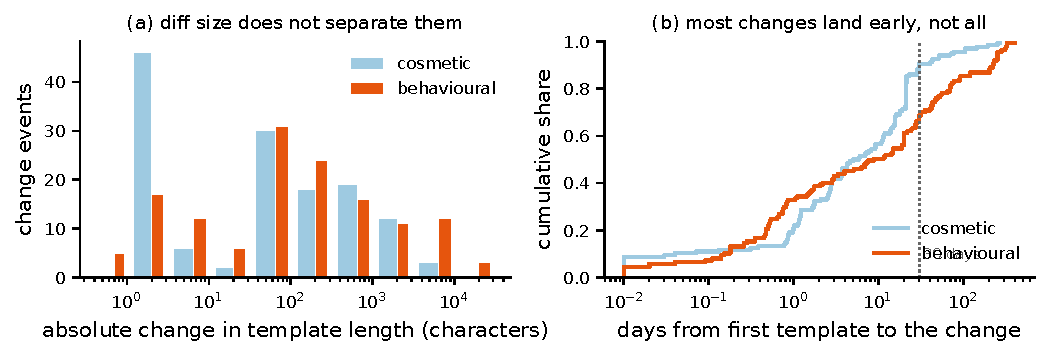
\includegraphics[width=\columnwidth]{fig1.pdf}
\caption{(a) The textual size of a template edit does not separate the edits that change what the
model sees from the ones that do not; the distributions overlap across four orders of magnitude.
(b) When the changes land, relative to a repository's first template. Most arrive within days, which
is why the paper reports a separate settled figure, but the tail extends well past a month.}
\label{fig:diffsize}
\end{figure}

\paragraph{Diff size does not tell you which is which.} % GENERATED by code/tables.py from the analysis output. Do not edit by hand.
Textual diff size is close to useless as a proxy: as a discriminator
between behavioural and cosmetic edits, the absolute change in template length achieves an AUC of
\DiffAUC{}, barely above chance. The median absolute
change in template length is \MedAbsLenCosmetic{} characters for cosmetic edits and
\MedAbsLenBehavioural{} for behavioural ones, and the distributions overlap heavily: the largest
purely cosmetic edit in the frame changes \MaxCosmeticLenChange{} characters and alters nothing the
model sees, while \NBehZeroLenChange{} behavioural edits change the template's length by zero. A
reviewer skimming a diff for size will misclassify both tails, which is the argument for deciding
this by rendering.

Figure~\ref{fig:diffsize}(a) shows the two distributions on top of each other.

\section{RQ2: does the model follow?}
\label{sec:rq2}

RQ1 established that renderings change. RQ2 asks whether the model's behaviour follows, which only
running the model can answer.

% GENERATED by code/tables.py from the analysis output. Do not edit by hand.
\begin{table}[t]
\caption{Same checkpoint, same conversation, same seed; only the historical chat template differs.
Checkpoint names drop their Instruct token for width; full identifiers are in
Section~\ref{sec:exec}.
\emph{Floor} is the response divergence between two runs of the \emph{same} template, a single
re-run of each checkpoint's first template: the serving stack's reproducibility noise for that
checkpoint. Resolution is the share of \NTasksExec{} repair tasks whose returned program passes its
test; contract is the share of replies obeying the stated output contract.
\textsuperscript{$\dagger$}~this template refuses the conversation outright: it raises on a system
message, so all \MistralRenderErr{} tasks fail before the model is reached.}
\label{tab:rq2}
\small
\begin{tabular}{lrlrr}
\toprule
checkpoint & floor & template & resolved & contract \\
\midrule
Mistral-7B-v0.2 & 0.0\% & 2023-12-11 & 0.0\%\,\textsuperscript{$\dagger$} & 0.0\% \\
 &  & 2024-07-03 & 28.3\% & 100.0\% \\
\addlinespace
Phi-3-mini-4k & 0.0\% & 2024-04-22 & 21.7\% & 90.0\% \\
 &  & 2024-04-29 & 10.0\% & 45.0\% \\
 &  & 2024-07-01 & 23.3\% & 88.3\% \\
\addlinespace
deepseek-coder-6.7b & 90.0\% & 2023-11-01 & 40.0\% & 98.3\% \\
 &  & 2023-11-01 & 43.3\% & 98.3\% \\
 &  & 2023-11-04 & 43.3\% & 96.7\% \\
 &  & 2023-11-28 & 45.0\% & 95.0\% \\
 &  & 2023-11-29 & 45.0\% & 98.3\% \\
 &  & 2023-12-13 & 45.0\% & 98.3\% \\
\addlinespace
Qwen2.5-7B & 15.0\% & 2024-09-16 & 28.3\% & 40.0\% \\
 &  & 2024-09-18 & 28.3\% & 40.0\% \\
\addlinespace
Meta-Llama-3-8B & 26.7\% & 2024-04-18 & 43.3\% & 100.0\% \\
 &  & 2024-04-19 & 43.3\% & 100.0\% \\
 &  & 2024-04-30 & 43.3\% & 100.0\% \\
\bottomrule
\end{tabular}
\end{table}


Table~\ref{tab:rq2} reports every checkpoint, its replication floor, and the two outcomes under each
of its historical templates.
Across \NCheckpoints{} checkpoints and \NExecEpisodes{} episodes, \NUninformative{} of the template
pairs turned out to render \emph{this} conversation identically despite differing on the probe set,
because the edit only touches a branch this conversation does not take. Those pairs vary nothing and
are excluded: an identical input producing an identical output is not evidence that the edit was
harmless. That leaves \NFamily{} informative comparisons, and both outcome families are
Holm-corrected across all \NFamily{}.

\paragraph{The floor first, because it disqualifies the obvious metric.} Running the same template
twice, byte-identical prompt and settings, changes the reply on \MinNoiseFloor\% of tasks for
\ShortMistral{} and \ShortPhi{} but on \MaxNoiseFloor\% for \ShortDS{}. Response divergence is
therefore useless as a drift signal on its own, since on \ShortDS{} it is near-saturated before any
template changes at all. What survives replication is the executed outcome, and that is what we test.

\paragraph{A template edit can make the request impossible.} \ShortMistral's original template
raises on a system message. All \MistralRenderErr{} tasks fail before the model is reached, giving
resolution \ResMistralA\% and contract compliance \ConMistralA\%. A later edit to the same
repository, on the same weights, accepts system messages: resolution \ResMistralB\% and contract
\ConMistralB\%. This is the one resolution comparison that survives Holm across all \NFamily{} tests
($p_{\text{Holm}}=\MistralPHolmRes$; the contract swing also survives, at
$p_{\text{Holm}}\,{\MistralPHolmCon}$), and it is categorical rather than statistical. A pipeline
pinned to the earlier revision cannot send a system prompt at all, and one written against the later
revision fails completely if it pulls the earlier one.

\paragraph{A template edit can halve what a prompt suite asserts, and a later edit can restore it.}
This is the strongest execution-grounded effect we observe, and it is a one-repository case study:
it establishes that the failure occurs, not how often. On \ShortPhi{}, contract compliance runs
\ConPhiA\%, then \ConPhiB\%, then \ConPhiC\% across the
repository's three templates, while resolution runs \ResPhiA\%, \ResPhiB\%, \ResPhiC\%. Both
contract transitions survive correction, down at $p_{\text{Holm}}\,{\PhiPHolmConDown}$ and back up
at $p_{\text{Holm}}\,{\PhiPHolmConUp}$. The size of the swing is the operational point rather than the
p-value: compliance halves at one edit and is restored at the next, a movement far outside the
checkpoint's own replication floor. The middle template is the commit whose own message describes
replacing the system role with the user role, which is what a halved compliance rate on a
system-carried output contract looks like from the outside. The resolution swing over the same two
transitions is large but does not survive correction across \NFamily{} tests
($p_{\text{Holm}}=\PhiPHolmResDown$ and \PhiPHolmResUp); with only \PhiDiscDown{} and \PhiDiscUp{}
discordant tasks the smallest p-value these exact tests can produce cannot clear a family of
\NFamily{}, so the design is underpowered for these transitions and we report them as suggestive
rather than as established or refuted.

\paragraph{This is where a then-versus-now check fails.} Comparing \ShortPhi's first template with
its last gives $p_{\text{Holm}}=\PhiFirstLastRes$ on resolution and a contract rate back to roughly
where it started. The repository broke and then repaired itself. A check that compares only the
current template against the one it was pinned at sees nothing, while what a consumer lived through
was the window in between.

\paragraph{Drift is often harmless.} \ShortDS{} ships \NVersDSCoder{} distinct
templates and none of the \NDSPairs{} informative comparisons between them moves resolution detectably, the
smallest being $p_{\text{Holm}}=\DSMinP$, with resolution staying between \ResDSCoderA\% and
\ResDSCoderF\%. Of the \NFamily{} informative comparisons, \NSigRes{} survives correction on
resolution and \NSigContract{} on contract compliance. The claim is not that template edits usually
break things. It is that some do, that the ones that do cannot be told from the ones that do not
without running the model, and that nothing in the tooling available when this study was run tells
a consumer which kind has just landed.

\paragraph{Two robustness checks, because both cut against us if they fail.} First, the excluded
uninformative pairs are put back and everything is re-corrected over all \NAllPairs{} pairs. This is
the \emph{more} conservative direction, since each restored pair contributes $p=1$ by construction
and enlarges the family, and the counts are unchanged: \NAllSigRes{} on resolution and
\NAllSigCon{} on contract. Second, each effect is read against its own checkpoint's replication
discordance. \ShortPhi{} and \ShortMistral{} show \FloorDiscPhi{} and \FloorDiscMistral{}
discordant tasks when a
template is replayed against itself, against \PhiDiscDown{} and \PhiDiscUp{} for the two \ShortPhi{}
transitions and \MistralDisc{} for \ShortMistral{}, so those effects sit well outside their own
noise. \ShortMistral's floor is trivially clean, since its replicated arm fails to render every
task; its effect rests on the categorical contrast above, not on that floor. \ShortQwen{} is the cautionary case in the other direction: replaying an identical prompt
moves its resolution enough that the replication arm would itself test significant
($p=\QwenFloorP$) against a zero-discordance null. Any single comparison on a checkpoint like that
should be disbelieved, which is precisely why the floor is measured rather than assumed.


\subsection{What actually changed}
\label{sec:mechanism}

Neither effect above needs a subtle explanation. Both are visible in the template source, and we give
them here because the mechanism is what makes the result actionable rather than anecdotal.

\ShortPhi's second template deletes one branch of the role dispatch. The earlier template handles
three roles:

{\small\begin{verbatim}
{% if (message['role'] == 'system') %}...
{% elif (message['role'] == 'user') %}...
{% elif message['role'] == 'assistant' %}...
\end{verbatim}}

\noindent The later one handles two, and the \texttt{system} arm is simply gone. A system message
therefore matches no branch and is emitted nowhere: it is discarded in silence, with no error and no
warning. Our system message is where the output contract lives, which is why contract compliance
falls to \ConPhiB\% and recovers when a subsequent edit restores the role.

\ShortMistral's original template is stricter and fails louder, though only at the point of
rendering:

{\small\begin{verbatim}
{% else %}{{ raise_exception(
  'Only user and assistant roles are supported!') }}
\end{verbatim}}

\noindent Any system message raises before a single token reaches the model. The later template
accepts one. So the same repository, at two revisions, is the difference between a system prompt
being impossible and a system prompt being ordinary, with no version number anywhere between them.

Both are one-branch edits. Neither changes a weight. Neither announces itself.

\subsection{A control that could have refuted us}

Both effects above involve the system role, so the mechanism implies a prediction that can fail: move
the output contract out of the system message and into the user turn, and the damage should
disappear. That prediction is the falsification criterion fixed in the design. We recorded it
before running the control, which repeats the study, the same tasks, decoding and grading, with a
system-free conversation, on the two checkpoints that produced an effect, \NSFEpisodes{} more
episodes. The control measures its own replication floors, \SFFloorMistral\% and \SFFloorPhi\%
response divergence; the latter differs from the main run's \FloorPhi{}\% for the same checkpoint,
which is why floors are measured per run rather than assumed.

Both predictions hold. \ShortMistral's earlier template raises on a system message and nothing else,
so with no system message it renders every task: render errors fall from \MistralRenderErr{} to
\NSFRenderErrors{}, and both of its templates now resolve \SFResMistralA\% with \SFConMistralA\%
contract compliance. The gap is gone. On \ShortPhi{}, contract compliance becomes \SFConPhiA\%,
\SFConPhiB\% and \SFConPhiC\% across the same three templates, so the collapse at the middle template
is gone as well. Of the \NSFFamily{} informative comparisons in the control, \NSFSigRes{} survive
correction on resolution and \NSFSigCon{} on contract compliance.

One further check falls out of the design rather than being asked for. With no system message,
\ShortPhi's first two templates render this conversation \emph{identically}, so the comparison
becomes uninformative by the same rule used throughout. That is deductive, not statistical: the two
templates differ only in the \texttt{system} arm of their role dispatch, shown in
Section~\ref{sec:mechanism}, so removing
the system role removes the entire difference between them.

\paragraph{Is this a role effect or merely a position effect?} Moving an instruction also moves it,
so the control changes two things at once and the recovery could in principle be the contract landing
somewhere more effective rather than landing at all. Two things rule that out.

First, under the templates that fail there is no instruction to reposition. Searching the rendered
prompt for the contract sentence finds it under \ShortPhi's first and third templates and \emph{not}
under its second: the deleted \texttt{system} arm means the text is emitted nowhere. \ShortMistral's
earlier template does not render at all. The contrast is presence against absence, not one position
against another.

Second, if position mattered independently, moving the contract would shift outcomes on templates
that handle the system role correctly (operationally, among the two checkpoints re-run
system-free, those whose main-run arm renders every task and keeps the contract satisfied on most
replies). The shifts there are small: across the \NHealthyTemplates{} such
templates here, moving the contract into the user turn changes resolution by at most
\MaxHealthyResShift{} points and contract compliance by at most \MaxHealthyConShift{}; \ShortMistral's
later template is unchanged on both, at \ResMistralB\% and \ConMistralB\%. The recovery appears only
where the template mishandles the role, which is what a role effect predicts and a position effect
does not.

The mechanism is therefore not ``the template changed'' in general. It is ``the template changed how it
handles the role your contract lives in''. That is a smaller claim than the one we could have made
from the main run alone, and it is the one the data supports. It also yields the mitigation a
practitioner can act on directly, in Section~\ref{sec:check}: if you cannot pin the template, do not put
load-bearing instructions in a system message. For instructions that must stay in the system role
for other reasons, safety and injection resistance among them, pinning the template is the
remaining defence.

\section{RQ3: pinning what a template renders}
\label{sec:check}

RQ1 counted the edits and RQ2 showed that some of them matter; RQ3 asks for a check that separates
the two at build time.

\NEvents{} template edits in this frame would each trip a check that hashes the template text, and
about half of the decidable ones render identically. An alert channel that is half
noise is muted, and a muted control is not a control.

\textsc{templatelock} pins a model by two values: the SHA-256 of its template, and a
\emph{render signature}, the hash of what that template produces on the six probe conversations. A
build that finds a new template hash but the same render signature reports a cosmetic change and
passes. A build that finds a new render signature reports a behavioural change and fails, because
what the model is shown has changed and the prompt evaluations no longer describe the deployed
system. A probe that fails to render contributes its error to the signature, so an edit that
breaks a probe that previously rendered also fails the build, and a pair whose two revisions fail
with different errors would alert as well. The replay below excludes the \NEventsUndecidable{}
events where neither revision renders from the alert accounting, tallying them separately, neither
raised nor suppressed. The signature is defined relative to a pinned rendering stack, so a team upgrading
its templating library re-pins at the upgrade, deliberately rather than silently.

The probe set is a parameter rather than a constant. A team whose traffic exercises serialisation
paths our six probes do not, tool calls above all, can append its own probe conversations, and the
render signature then covers exactly the shapes that team depends on. A probe is one fixed message
list, so extending the set costs milliseconds.

Replayed over the frame's histories, a plain template hash raises \NaiveAlerts{} alerts;
\textsc{templatelock} raises \RenderAlerts{} and holds back \SuppressedAlerts{}
(\PctSuppressed\% of decidable events) as cosmetic. A pipeline that pinned at a model's first
template and never re-pinned would have ended on a rendering different from the one it validated
against in \NStranded{} repositories, first diverging after a median of \MedianDaysStranded{} days.

How does this differ from pinning a commit SHA? A team that pins its model repository to a commit,
which Hub tooling supports but does not do by default, prevents silent drift entirely, and a team
that can freeze its dependency should. What a SHA pin cannot do is classify: it blocks the cosmetic
majority of edits along with the behavioural ones, so it either freezes the pipeline out of
upstream fixes or, when the pin is eventually moved, says nothing about whether the jump matters.
\textsc{templatelock} is the complement rather than the rival: it tells a team when moving the pin
is safe.

The cost is the reason to adopt it rather than discuss it: \CostComputeMs{} ms per model for six
renders and a hash, on top of a tokenizer load a build already performs. That is one wall-clock
measurement on one machine and is the only number here that does not reproduce exactly; what
transfers is the order of magnitude, milliseconds against a network fetch.

\section{Threats to validity}

\paragraph{The probe set bounds what we can call behavioural.} Six conversations cannot exercise
every path through a Jinja template, and they are six conversations rather than six independent
shapes: two of them, the bare coding request and the reply-with-one-word probe, are each a single
user turn with the generation prompt requested, differing only in
content, and they fire on the same number of pairs. Tool-call and structured-output serialisation,
already a large part of what templates encoded at the time of this study, are not probed at all,
and neither are the reasoning segments some model families encode. A template edit touching only those
paths is scored cosmetic here. Every one of these gaps biases the behavioural rate \emph{downward},
so \PctEventsBeh\% is a lower bound on the fraction of decidable edits that change what the model
is shown, not an estimate of the fraction that changes behaviour. \textsc{templatelock} is also not an
adversarial defence: its probes are fixed and public, so an edit crafted to render them
identically while changing other paths would pass it by construction.

\paragraph{Weight-silence depends on recognising a weight file.} The classifier keys on file
extension, so a weight shipped under an unrecognised one would be counted as silence. We checked
rather than assumed: across all weight-silent intervals in the frame, the extensions that do change
are configuration, documentation and template files, and \emph{no} model-weight extension appears
in any of them. Extending the list to further formats leaves every figure in this section unchanged.

\paragraph{Rendering divergence is necessary, not sufficient.} A rendering can differ by a single
whitespace character and leave the model's output untouched. This is why RQ2 exists and why it is
read against a replication floor: RQ1 alone would establish only that the input changed.

\paragraph{The checkpoints are quantised, and one repository is a mirror.} Local checkpoints are
quantised rather than the Hub's full-precision weights. Quantisation is held fixed across arms, so it
cannot confound a within-checkpoint comparison, but the magnitude of an effect on full-precision
weights may differ. The official Llama-3 repository is gated and cannot be read anonymously, so its
template history is taken from a public mirror of the same checkpoint
(NousResearch/Meta-Llama-3-8B-Instruct), whose commit history records the mirror's uploads rather
than the upstream repository's edits.

\paragraph{Repair is one task family, and the probe set is six conversations.} RQ2 measures
single-function program repair in Python, and the cosmetic/behavioural split is decided on six fixed
probe conversations. Every behavioural claim here should be read as established on that basis and
not beyond it: we have not tested tool calling, retrieval-augmented prompts, long multi-turn
sessions, or any non-Python domain, and a template edit that damages one of those would be invisible
to this study. In a domain without an execution oracle, summarisation or open-ended reasoning, the
same mechanism would surface differently. A dropped system role discards whatever the system message
carried, a style constraint or a safety instruction rather than an output contract, and the
degradation would be visible only to a judge, human or model, rather than to a test suite.

\paragraph{The one surviving resolution effect is a rendering failure, not a degraded model.}
\ShortMistral's earlier template refuses the conversation, so its resolution difference measures a
request that could not be sent rather than a model answering worse. Among comparisons where the
model did receive a prompt, no resolution difference survives correction. We report task
consequence as not established rather than as absent: the uncorrected bootstrap intervals for the
two \ShortPhi{} transitions (earlier arm minus later, \PhiCIDownLo{} to \PhiCIDownHi{} and
\PhiCIUpLo{} to \PhiCIUpHi{}
resolution points) lie on one side of zero, so the corrected nulls reflect the tests' resolving
power at these discordance counts, not evidence of no effect.
The evidence that a template edit changes behaviour on valid input
rests on output-contract compliance, one of the properties a prompt suite asserts, and not on task
outcome. That evidence comes from one repository of the \NCheckpoints{} we ran, so it establishes
that the effect occurs and not how often it does: on valid input this half of RQ2 is a case study,
and we do not read a rate from it.

\paragraph{Popularity-ranked frames are not random samples.} The frame is the head of the download
distribution, where maintainers are most active and most scrutinised. The out-of-frame extension
suggests a lower rate further down, and we report it separately rather than pooling. Download rank
also measures pulls rather than production dependence: \NFixtures{} of the \NFrame{} repositories
are recognisable test fixtures (tiny, dummy or random checkpoints). Excluding them leaves the drift rate unchanged, moves the settled figure from
\PctBehSettledFrame\% to \PctBehSettledNoFix\%, and moves the behavioural share of decidable
events from \PctEventsBeh\% to \PctEventsBehNoFix\%. Follow-up is also heterogeneous: a repository
whose first template is younger than \SettledDays{} days cannot yet enter the settled numerator
while it stays in the denominator, so the settled figure is, if anything, understated.

\paragraph{We make no claim that maintainers acted wrongly.} Many of these edits are corrections, and
correcting a broken template is good practice. The finding is not that the edits are bad. It is that
consumers cannot see them happen.

\section{Related work}

Prompts as evolving software artifacts have been studied by mining repositories: an analysis of
\lit{1{,}262} prompt changes across \lit{243} projects finds prompt edits poorly documented, with
only \lit{21.9}\% explained in commit messages~\cite{tafreshipour2024prompting}. That work studies
the prompt text an application owns. We study the artifact between that text and the model, which
the application does not own and usually cannot see.

Vibe coding has so far been characterised qualitatively: a grey-literature review of \lit{101}
practitioner sources~\cite{fawzy2026vibepractice} and a survey of \lit{162}
participants~\cite{fawzy2026verification} both describe a practice in which output is judged by
running it and quality assurance is often skipped. Those studies establish that the verification
loop is thin. We measure a dependency that such a loop is structurally unable to see.

Dependency drift is old ground in software engineering. In npm, around \lit{12}\% of dependent
packages were affected by breaking changes during non-major updates, and \lit{44}\% of manifesting
breaking changes arrived in minor and patch releases~\cite{venturini2023depended}. The chat-template
case is the same hazard with the versioning removed. Documentation-side artifacts such as model
cards~\cite{mitchell2019modelcards} describe a model for humans; the chat template configures it for
machines, and only the latter changes what is computed.

That a model's output is sensitive to formatting is established rather than novel, and it is what
makes this dependency worth versioning. Semantically neutral formatting changes move accuracy by up
to \lit{76} points on one open model~\cite{sclar2024formatspread}. Hosted services drift
behaviourally between releases without announcing what changed~\cite{chen2023chatgptdrift}. Our
contribution is not that format matters; it is that on open weights the formatting artifact is a
file in the repository, it is edited in place with no version, and both the edits and their
behavioural consequences can therefore be measured directly rather than inferred from a black box.

Work on repair loops asks what feedback to put into the next
turn~\cite{olausson2024selfrepair,ray2026structured,iscan2026falsification}. That literature holds
the serialisation fixed and varies the content. We hold the content fixed and vary the
serialisation.

\section{Conclusion}

A prompt pipeline that versions its prompts and pins its model still depends on an executable
artifact it does not version and cannot see. In \NFrame{} of the most-downloaded open-weight chat
repositories, \PctDrifted\% edited that artifact after release, half of the decidable edits changed
what the model is shown, and \PctEventsWeightSilent\% of edits happened while no weight file moved.
Much of that raw rate is launch-week churn; the figure to carry is that \PctBehSettledFrame\% of the
frame (\PctBehSettledNoFix\% excluding the test fixtures disclosed above) changed what the model is
shown more than \SettledDays{} days after first publishing a
template.
Running \NCheckpoints{} checkpoints under their own historical templates, \NSigContract{} of
\NFamily{} informative comparisons move output-contract compliance after correction; the two on
valid input are the case-study repository's, and the third is the render-refusal pair, which is
also the only comparison that moves task resolution. On valid input we find no surviving resolution effect and say so. Others drift with no
measurable effect, which is the difficulty rather than a reassurance: from outside the repository the
two look identical. A pre-registered control locates the mechanism in the system role, since moving
the contract into the user turn removes both failures, which gives practitioners something to do
about it besides worry.

Pinning what a template renders, rather than what it says, separates the edits that matter from the
ones that do not at a cost of \CostComputeMs{} ms per model. Prompt CI cannot claim to pin the model's input
until it versions the template too.

\section*{Data availability}

The collector, the renderer, the full template histories of the frame, the execution episode log,
the analysis code and \textsc{templatelock} are released at
\url{https://github.com/s1mar/chat-template-drift} (release tag \texttt{cr-1.0}). The package
reproduces every deterministic number in this paper from the recorded histories, without network
access; the single wall-clock cost figure transfers in order of magnitude only.


\balance
\bibliographystyle{ACM-Reference-Format}
\bibliography{refs}

\end{document}
